%%%%%%%% ICML 2018 EXAMPLE LATEX SUBMISSION FILE %%%%%%%%%%%%%%%%%

\documentclass{article}

% Recommended, but optional, packages for figures and better typesetting:
\usepackage{microtype}
\usepackage{graphicx}
\usepackage{subfigure}
\usepackage{booktabs} % for professional tables

% hyperref makes hyperlinks in the resulting PDF.
% If your build breaks (sometimes temporarily if a hyperlink spans a page)
% please comment out the following usepackage line and replace
% \usepackage{icml2018} with \usepackage[nohyperref]{icml2018} above.
\usepackage{hyperref}

% Attempt to make hyperref and algorithmic work together better:
\newcommand{\theHalgorithm}{\arabic{algorithm}}

% Use the following line for the initial blind version submitted for review:
\usepackage[accepted]{icml2018}

% If accepted, instead use the following line for the camera-ready submission:
%\usepackage[accepted]{icml2018}

% The \icmltitle you define below is probably too long as a header.
% Therefore, a short form for the running title is supplied here:
\icmltitlerunning{Submission and Formatting Instructions for ICML 2018}

\begin{document}

\twocolumn[
\icmltitle{Replication Review for Coordinated Exploration in
Concurrent Reinforcement Learning}


\icmlsetsymbol{equal}{*}

\begin{icmlauthorlist}
\icmlauthor{Ed Fancher}{su}
\end{icmlauthorlist}

\icmlaffiliation{su}{Department of Computer Science Stanford University, Stanford, California}

\icmlcorrespondingauthor{Ed Fancher}{efancher@stanford.edu}

% You may provide any keywords that you
% find helpful for describing your paper; these are used to populate
% the "keywords" metadata in the PDF but will not be shown in the document
%  \icmlkeywords{Machine Learning, ICML}

\vskip 0.3in
]

% this must go after the closing bracket ] following \twocolumn[ ...

% This command actually creates the footnote in the first column
% listing the affiliations and the copyright notice.
% The command takes one argument, which is text to display at the start of the footnote.
% The \icmlEqualContribution command is standard text for equal contribution.
% Remove it (just {}) if you do not need this facility.

%\printAffiliationsAndNotice{}  % leave blank if no need to mention equal contribution
\printAffiliationsAndNotice{} 
% otherwise use the standard text.

\begin{abstract}
This is a replication attempt for a a paper on seed sampling. Seed sampling is a way to provide a stable and efficient mechanism for exploring the state action space for multi-agent reinforcement learning algorithms. In the replicated paper, 3 exploration methods are compared, using a common multiple agent learning algorithm : Upper Control Bounds,  Thompson Sampling, and Seed Sampling.

\end{abstract}

\vskip 1.0in
\section{Introduction}
There are multiple approaches to exploration in single agent settings. These approaches may not always extend well to multiple agent settings. There are 2 single agent methods which have had some success: Upper Control Bound \cite{UCB2010} and PSRL (Bayesian) methods \cite{Strens2000}
In this project, I attempt to replicate the findings in \cite{SeedSampling}. In this paper 3 approaches are compared: UCB based multiple agent approaches, Thompson Sampling and Seed Sampling. Seed Sampling is based on the single agent PSRL approach.  In the UCB approach, as presented in the paper, the agents do not coordinate directly on exploration. Instead, they maintain a shared model and at each time step will calculate the best approach based on that model using an upper control bound. 

In the Thompson Sampling approach, at each time step, a potential MDP is constructed on the transitions and/or Rewards, based on transitions/rewards seen up to this point. Each agent then samples independently from the MDP to take the next step. In seed sampling, an MDP is constructed at the beginning of each episode, similarly to Thompson Sampling, and this is used to generate a policy for the episode. So the main difference between Thompson Sampling and Seed Sampling is that seed sampling samples per episode, and Thompson Sampling samples per time step.

An important consideration is that, in terms of the paper's construction of the problem, an MDP (could be an approximation) must be solved for all three methods. For UCB and Seed Sampling, it's done once per episode, for Thompson Sampling it's every time step.

Each set of three approaches is tested on three simple problems.

1) A bipolar chain, constructed as $-10 \longleftrightarrow -1 \longleftrightarrow ... \longleftrightarrow -1 \longleftrightarrow 10$. The chain can be reversed. So there are 3 rewards: -10, 10, -1 and 2 actions: left, right. All transactions are deterministic. The -10 and 10 states are also stopping states.

Here is an image from the paper showing a bipolar chain:

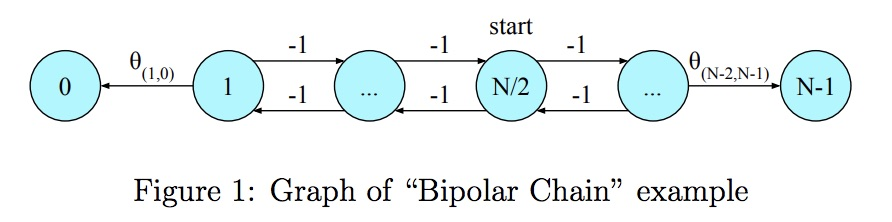
\includegraphics[scale=.2]{bipolarchain.jpg}

2) Parallel chains, constructed as a a set of linked lists with a common node at one end. All nodes have 0's except the the end nodes. Those have arbitrary unique rewards.

Here is an image from the paper showing a set of parallel chains:

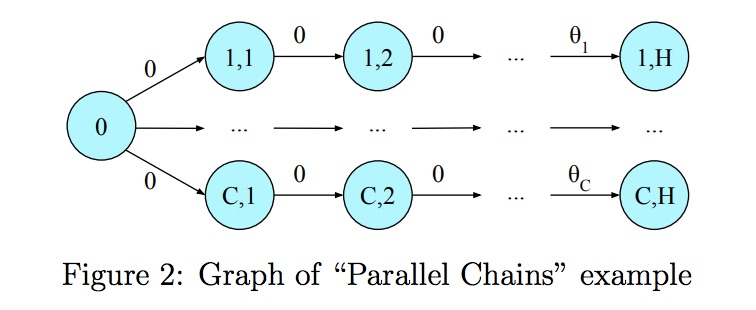
\includegraphics[scale=.2]{parallelchains.jpg}

3) Maximum reward path. This is constructed as a graph with nodes connected with probability p and rewards that are normally distributed.

\section{Background/Related Work}

\section{Approach}
Although this is a multiple agent problem, the Seed Sampling paper treated actions as occurring within discrete time steps, so it wasn't necessary to use a distributed (including multi-threaded) approach. So, I decided to take advantage of the fairly nice POMDP.jl framework in Julia. 

Steps:

  \begin{itemize}
  
\item Solve the true MDP using some method. I've been using Q-learning with e-greedy so far.
  
\item Use the POMDP.jl methods to run a simulation on the problem, providing a function policy that matches the exploration method. For the chain, this stops as soon as it hits a goal state. For the other two, likely a complete exploration will be necessary.

Each successive time step will see a new agent started, so if there are k agents, there would be one agent started at each time step $t_1$, $t_2$, ..., $t_k$.
\item Repeat for multiple runs, stepping through different \#'s of agents. Calculate the average regret.

  
  Currently I have all three exploration methods working for the chain MDP.
  
 \end{itemize}
  Next steps:
  \begin{itemize}
\item Do a full run for bipolar chain with 100 states and a horizon of 150, per the Seed Sampling paper.

I expect to start this right after assignment 3 is due.

\item Repeat for parallel chains

This should be a relatively straight forward update from the bipolar chain.  

I expect to start this within a day of the assignment 3 deadline.

\item Repeat for Maximum reward path (likely the most difficult)

This one will likely be more complicated since there are a much larger possible number of actions. I expect to start this by March 6th

\item Various items to handle reporting and graphing (probably in R). Hopefully a few days before the 20th. :)

\item Final report.
 \end{itemize}

    
\section{Experiment results}
I have done runs with a short 20 node bipolar chain for all three exploration types for 1, 2, 5, and 10 agents.
\begin{tabular}{|c|c|c|}
\hline 
algorithm & agents & average regret \\ 
\hline 
Seed Sampling & 1 & 25.4 \\ 
\hline 
Seed Sampling&2&20.1 \\ 
\hline 
Seed Sampling&5&17.6 \\ 
\hline 
Seed Sampling&10&15.2 \\ 
\hline 
Thompson Sampling&1&40.6 \\ 
\hline 
Thompson Sampling&2&40.6  \\ 
\hline 
Thompson Sampling&5&35.78 \\ 
\hline 
Thompson Sampling&10&33.8  \\ 
\hline 
UCB&1&32.4  \\ 
\hline 
UCB&2&31.4 \\ 
\hline 
UCB&5&28.9 \\ 
\hline 
UCB&10&25.2 \\ 
\hline 
\end{tabular} 

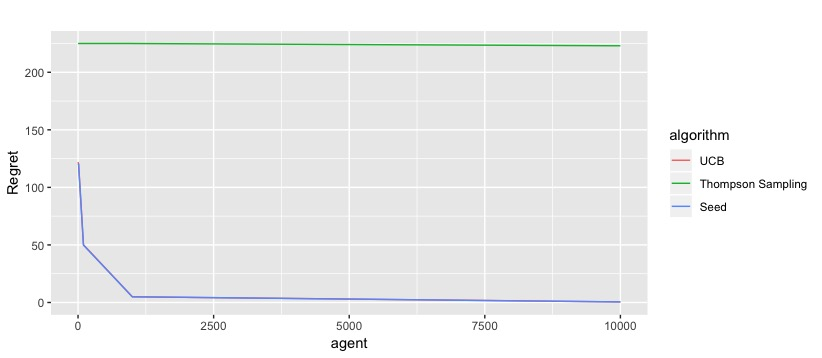
\includegraphics[scale=.6]{results_pre.jpeg}

There are some small discrepancies. Thompson sampling shows a drop for 5 and 10 agents, but I think this is likely due to the small chain size, which allows an agent to accidentally hit the end goal, with some higher than expected frequency. In addition, in the paper, UCB was a little closer to the performance of Seed Sampling. This could be that the paper was a little vague about the parallel UCB algorithm used. I implemented a version of UCB1 that used Q and N tables that were common across the agents. Despite this, the improvement when using Seed Sampling is still quite remarkable, and generally consistent with the improvement shown in the paper (if not better, really.)

\subsection{Parallel Chains}

\begin{table}[]
\begin{tabular}{|c|c|c|c|} 
\hline 
Seed Sampling     & 1       & 11.29179   \\ 
\hline 
Seed Sampling     & 10    & 13.4939681 \\ 
\hline 
Seed Sampling     & 100     & 5.3208811  \\ 
\hline 
Seed Sampling     & 1000   & 1.0470233  \\ 
\hline 
Seed Sampling     & 10000  & 0.4673821  \\ 
\hline 
Thompson Sampling & 1          & 14.2777303 \\ 
\hline 
Thompson Sampling & 10       & 12.70898   \\ 
\hline 
Thompson Sampling & 100    & 5.6677106  \\ 
\hline  
Thompson Sampling & 1000    & 1.0721236  \\ 
\hline 
Thompson Sampling & 10000  & 0.473994   \\ 
\hline 
UCB               & 1         & 18.813709  \\ 
\hline 
UCB               & 10       & 17.1507441 \\ 
\hline 
UCB               & 100      & 10.0549201 \\ 
\hline 
UCB               & 1000    & 1.4543679  \\ 
\hline 
UCB               & 10000  & 0.49      \\ 
\hline 
\end{tabular}
\end{table}
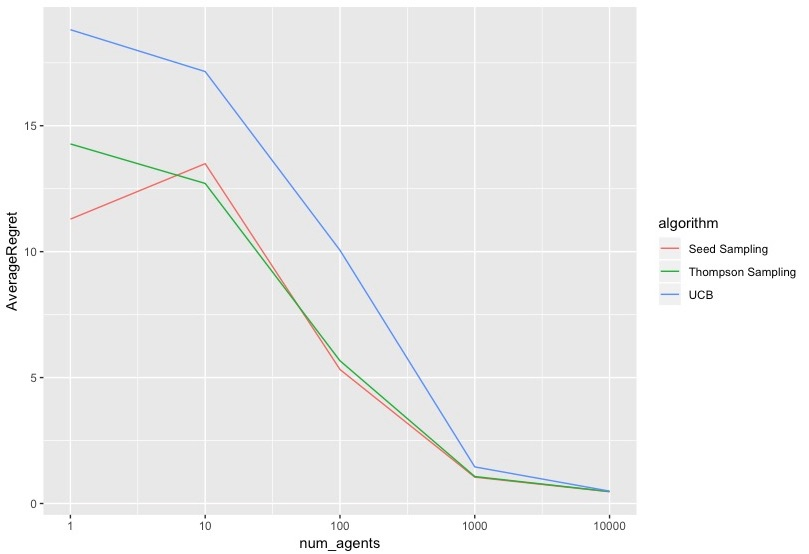
\includegraphics[scale=.3]{pc_results_regret_by_algo.jpg}
\section{Conclusion}

\section{References}

\bibliography{project_update}
\bibliographystyle{icml2018}



\end{document}


% This document was modified from the file originally made available by
% Pat Langley and Andrea Danyluk for ICML-2K. This version was created
% by Iain Murray in 2018. It was modified from a version from Dan Roy in
% 2017, which was based on a version from Lise Getoor and Tobias
% Scheffer, which was slightly modified from the 2010 version by
% Thorsten Joachims & Johannes Fuernkranz, slightly modified from the
% 2009 version by Kiri Wagstaff and Sam Roweis's 2008 version, which is
% slightly modified from Prasad Tadepalli's 2007 version which is a
% lightly changed version of the previous year's version by Andrew
% Moore, which was in turn edited from those of Kristian Kersting and
% Codrina Lauth. Alex Smola contributed to the algorithmic style files.
